\documentclass[notitlepage,cs4size,punct,oneside]{ctexrep}

% default paper settings, change it according to your word
\usepackage[a4paper,hmargin={2.54cm,2.54cm},vmargin={3.17cm,3.17cm}]{geometry}

\usepackage{amsmath,amssymb,amsthm}
\usepackage{titlesec}

% 公式编号的计数格式, 在章内计数
\numberwithin{equation}{chapter}

% set the abstract format, need abstract package

\usepackage[runin]{abstract}
\usepackage{algorithm}
\usepackage{algpseudocode}
\usepackage{booktabs}
\usepackage{graphicx}
\usepackage{float} % 图片和表格定位
\usepackage{subfigure} % 子图包
\usepackage{xcolor}





\usepackage[pdfborder={0 0 0},colorlinks=true,linkcolor=blue,CJKbookmarks=true, unicode=true]{hyperref}
%若要用LATEX编译, 请用下面的命令替代上述命令:
% \usepackage[dvipdfm,pdfborder={0 0 0},colorlinks=true,linkcolor=blue,CJKbookmarks=true]{hyperref}

\usepackage{mathrsfs}
\usepackage{longtable}

%\usepackage{boondox-calo}
%\usepackage{dutchcal}

\setlength{\absleftindent}{1.5cm} \setlength{\absrightindent}{1.5cm}
\setlength{\abstitleskip}{-\parindent}
\setlength{\absparindent}{0cm}

% Theorem style
\newtheoremstyle{mystyle}{3pt}{3pt}{\kaishu}{0cm}{\bfseries}{}{1em}{}
\theoremstyle{mystyle}
\usepackage{listings}
\lstset{
    language = Python,
    backgroundcolor = \color{yellow!10},    % 背景色:淡黄
    basicstyle = \small\ttfamily,           % 基本样式 + 小号字体
    rulesepcolor= \color{gray},             % 代码块边框颜色
    breaklines = true,                  % 代码过长则换行
    numbers = left,                     % 行号在左侧显示
    numberstyle = \small,               % 行号字体
    showstringspaces   =   false,
    keywordstyle = \color{blue},            % 关键字颜色
    commentstyle =\color{gray},        % 注释颜色
    stringstyle = \color{red!100},          % 字符串颜色
    frame = shadowbox,                  % 用(带影子效果)方框框住代码块
    showspaces = false,                 % 不显示空格
    columns = fixed,                    % 字间距固定
    %escapeinside={<@}{@>}              % 特殊自定分隔符:<@可以自己加颜色@>
    morekeywords = {with},                % 自加新的关键字(必须前后都是空格)
    deletendkeywords = {compile}        % 删除内定关键字;删除错误标记的关键字用deletekeywords删!
}


\newtheorem{definition}{\hspace{2em}定义}[chapter]
% 如果没有章, 只有节, 把上面的[chapter]改成[section]
\newtheorem{theorem}[definition]{\hspace{2em}定理}
\newtheorem{axiom}[definition]{\hspace{2em}公理}
\newtheorem{lemma}[definition]{\hspace{2em}引理}
\newtheorem{proposition}[definition]{\hspace{2em}命题}
\newtheorem{corollary}[definition]{\hspace{2em}推论}
\newtheorem{remark}{\hspace{2em}注}[chapter]
%类似地定义其他“题头“. 这里“注“的编号与定义、定理等是分开的

\def\theequation{\arabic{chapter}.\arabic{equation}}
\def\thedefinition{\arabic{chapter}.\arabic{definition}.}

% title - \zihao{1} for size requirement \bfseries for font family requirement
\title{{\zihao{1}\bfseries 期末作业:自监督训练、Transformer与三维重建}}
\author{何益涵 \quad 20307110032\\吕文韬 \quad 23210180109}

\date{}
%%%%%%%%%%%%%%%%%%%导言区设置完毕
%%%%%%%%%%%%%%%%%%%%%%%%%%%%%%%%%%%%%%%%%%%%%%%%%%%%%%%%%%%%%%%%%%%%%
\begin{document}
%Styles for chapters/section
%若要将章标题左对齐, 用下面这个语句替换相应的设置
%\CTEXsetup[nameformat={\raggedright\zihao{3}\bfseries},%
\CTEXsetup[nameformat={\zihao{3}\bfseries},
           format={\zihao{3}\bfseries\centering},
           beforeskip={0.8cm}, afterskip={1.2cm}]{chapter}
\CTEXsetup[nameformat={\zihao{4}\bfseries},
           format={\zihao{4}\bfseries\centering},
           name={第~,~节},number={\arabic{section}},
           beforeskip={0.4cm},afterskip={0.4cm}]{section}
\CTEXsetup[nameformat={\zihao{-4}\bfseries},
           format={\zihao{-4}\bfseries},
           number={\arabic{section}.\arabic{subsection}.},
           beforeskip={0.4cm},afterskip={0.4cm}]{subsection}
\CTEXoptions[abstractname={摘要: }]
\CTEXoptions[bibname={\bfseries 参考文献}]

\renewcommand{\thepage}{\roman{page}}
\setcounter{page}{1}
% \tableofcontents\clearpage

\maketitle\renewcommand{\thepage}{\arabic{page}}
\thispagestyle{empty}\setcounter{page}{0}
%%%  论文的页码从正文开始计数, 摘要页不显示页码
% 撰写论文的摘要
\renewcommand{\abstractname}{摘要: }
\begin{abstract}
     本项目的仓库地址为\href{https://github.com/HeDesertFox/Neural-Networks-and-Deep-Learning-Homework-Group-Tasks.git}{该超链接}\footnote{\href{https://github.com/HeDesertFox/Neural-Networks-and-Deep-Learning-Homework-Group-Tasks.git}{https://github.com/HeDesertFox/Neural-Networks-and-Deep-Learning-Homework-Group-Tasks.git}}. 详见其中的文件夹\texttt{final}.其中包含自监督框架任务\texttt{task1\_self\_supervised\_learning}、Transformer任务\texttt{task2\_Transformer\_vs\_CNN}和三维重建任务\texttt{task3\_object\_reconstruction\_view\_synthesis}.

     本项目提供了训练好的模型,详见\href{}{百度网盘}\footnote{提取码 },若链接失效,也可以通过 Github Issue 联系作者.


\end{abstract}



\chapter{对比监督学习和自监督学习在图像分类任务上的性能表现}
\section{任务描述}
\begin{enumerate}
\item 实现任一自监督学习算法并使用该算法在自选的数据集上训练ResNet-18,随后在CIFAR-100数据集中使用Linear Classification Protocol对其性能进行评测;
\item 将上述结果与在ImageNet数据集上采用监督学习训练得到的表征在相同的协议下进行对比,并比较二者相对于在CIFAR-100数据集上从零开始以监督学习方式进行训练所带来的提升;
\item 尝试不同的超参数组合,探索自监督预训练数据集规模对性能的影响.
\end{enumerate}

\section{项目架构}
\begin{enumerate}
    \item \texttt{data\_preparation.py}文件:
    \item \texttt{model.py}文件:
    \item \texttt{training.py}文件:
    \item \texttt{test\_notebook.ipynb}文件:
    \end{enumerate}

\section{实验设置}
\subsection{模型选择}
本项目的自监督训练框架是 SimCLR,\href{http://proceedings.mlr.press/v119/chen20j/chen20j.pdf}{详见以下论文}。
\begin{figure}[H]
    \centering
    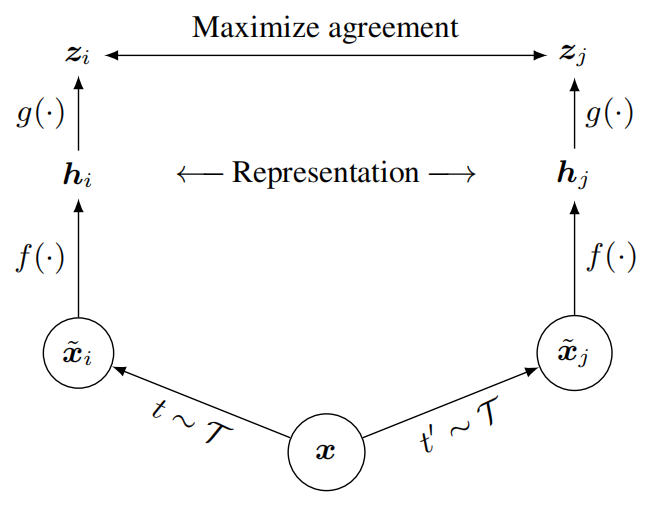
\includegraphics[scale=0.6]{simclr.png}
    \caption{SimCLR 架构}
    % \label{fig:fine}
\end{figure}
SimCLR 是一种用于自监督学习的框架,旨在学习高质量的视觉表示。其核心思想是通过对比学习来最大化正样本对之间的相似度,并最小化负样本对之间的相似度。SimCLR架构主要包括以下几个关键步骤:
\begin{enumerate}
\item 数据增强:SimCLR对每张输入图像应用一系列随机的数据增强操作(如裁剪、旋转、颜色抖动等),生成两种不同的视图。这些视图构成正样本对,而来自不同图像的视图构成负样本对。

\item 编码器:使用深度神经网络(通常是ResNet)作为编码器,将每个增强后的图像视图映射到一个低维特征空间中。编码器的输出是一个固定长度的特征向量。

\item 投影头(Projection Head):为了计算对比损失,SimCLR在编码器之后引入了一个小型的 MLP 投影头,将编码器的输出特征向量进一步映射到另一个特征空间中。这个步骤有助于学习更好的表示。

\item 对比损失(Contrastive Loss):SimCLR使用一种称为 NT-Xent(Normalized Temperature-scaled Cross Entropy)对比损失函数。对于每对正样本对,损失函数鼓励它们在特征空间中彼此接近,同时使负样本对之间的距离尽可能远。
\end{enumerate}

整个 SimCLR 框架通过在一个大规模未标注数据集上进行训练,逐步优化编码器和投影头的参数。经过训练后,编码器能够提取有用的图像特征,这些特征可以用于下游任务(如分类、检测等)。

SimCLR的一个显著优点是它仅依赖于数据增强和对比学习,无需任何人工标注的数据,从而有效利用大量未标注的数据进行训练。通过学习更加通用的特征表示,SimCLR 在许多视觉任务中表现出色,并成为自监督学习领域的重要方法之一。
\begin{figure}[H]
    \centering
    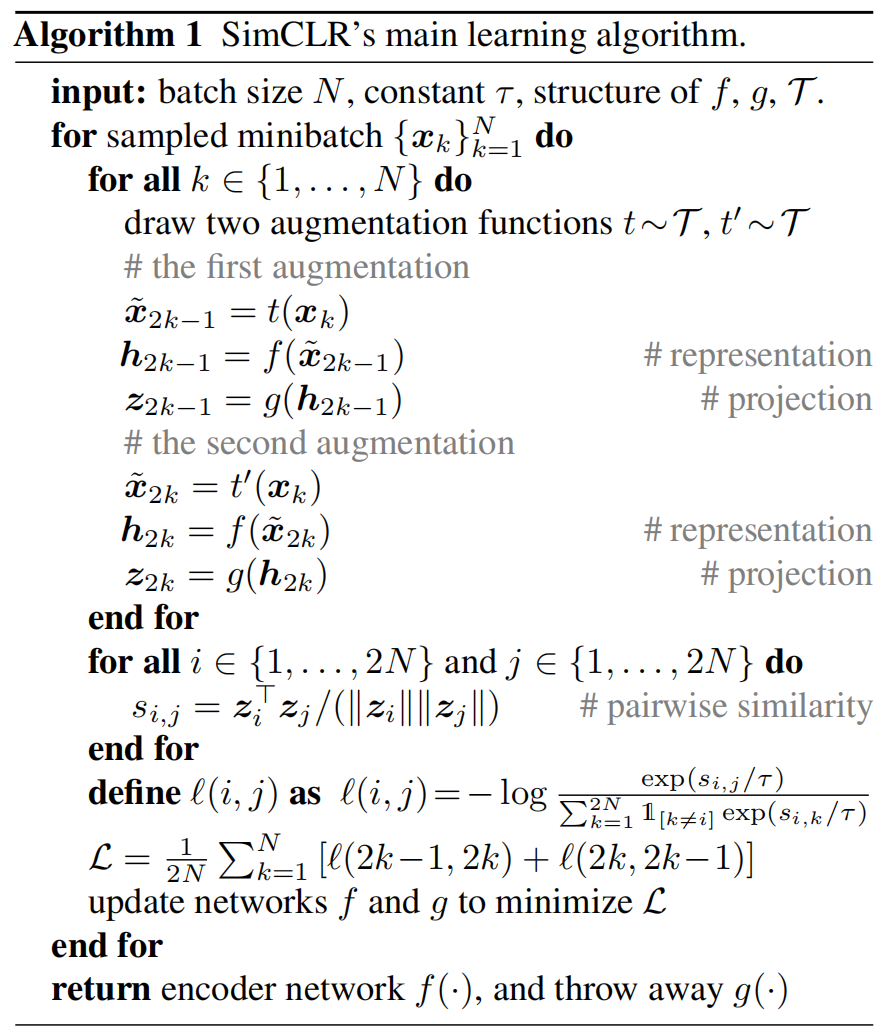
\includegraphics[scale=0.6]{simclr_code.png}
    \caption{SimCLR 伪代码}
    % \label{fig:fine}
\end{figure}

\subsection{数据集选择}

\subsection{优化器设置}

\section{实验结果}
\subsection{数据分析}

\chapter{在 CIFAR-100 数据集上比较基于 Transformer 和 CNN 的图像分类模型}
\section{任务描述}
\begin{enumerate}
\item 分别基于 CNN 和 Transformer 架构实现具有相近参数量的图像分类网络;
\item 在 CIFAR-100 数据集上采用相同的训练策略对二者进行训练,其中数据增强策略中应包含 CutMix;
\item 尝试不同的超参数组合,尽可能提升各架构在CIFAR-100上的性能以进行合理的比较。
\end{enumerate}


\section{项目架构}
此任务的所有文件在\texttt{task2\_Transformer\_vs\_CNN}文件夹中,其中包含以下文件:
\begin{enumerate}
\item \texttt{data\_preparation.py}文件:包含数据下载函数与预处理函数,其中包含 Cutmix 的实现.
\item \texttt{model.py}文件:包含 Resnet 和 ViT 的模型构造函数.
\item \texttt{training.py}文件:包含训练和超参数调优函数.
\item \texttt{test\_notebook.ipynb}文件:包含 Transformer 架构和 CNN 架构的对比任务的全部流程,如数据加载、调参和训练可视化.
\end{enumerate}

\section{实验设置}
\subsection{数据增广}
此项目的数据增广在常规图像变化的基础上增加了 Cutmix 增强方法。\href{http://openaccess.thecvf.com/content_ICCV_2019/papers/Yun_CutMix_Regularization_Strategy_to_Train_Strong_Classifiers_With_Localizable_Features_ICCV_2019_paper.pdf}{详见以下论文}。

CutMix是一种数据增强技术,旨在提升网络的泛化性能。CutMix的主要思想是在训练图像之间剪切并粘贴图像块,同时按比例混合相应的标签。此方法有助于模型从更多样化的训练样本中学习,从而提高其鲁棒性和性能。

CutMix的原理包括两个主要步骤:从一张图像中剪切出一个块并将其粘贴到另一张图像上,然后按比例调整两张图像的标签。具体来说,对于两张图像 $x_A$ 和 $x_B$ 及其对应的标签 $y_A$ 和 $y_B$,新的图像 $\tilde{x}$ 和标签 $\tilde{y}$ 的生成方式如下:
\begin{equation}
\tilde{x} = M \odot x_A + (1 - M) \odot x_B
\end{equation}
\begin{equation}
\tilde{y} = \lambda y_A + (1 - \lambda) y_B
\end{equation}
其中,$M$ 是一个二进制掩码,表示图像块的应用位置,$\odot$ 表示元素级乘法,$\lambda \in [0, 1]$ 是表示原始图像保留比例的随机变量,通常从Beta分布中采样。
\begin{figure}[H]
    \centering
    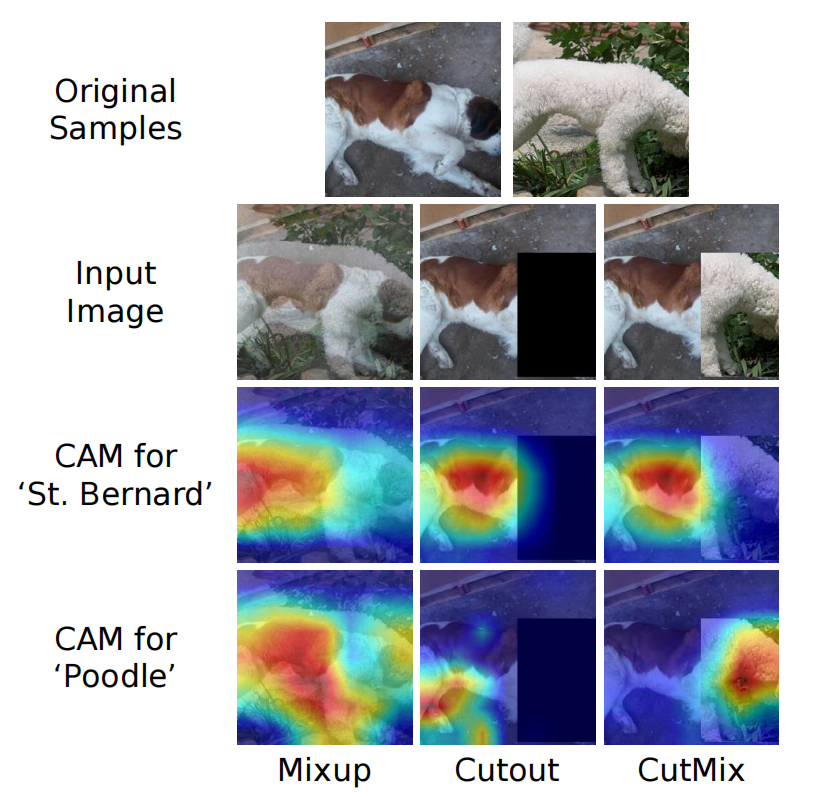
\includegraphics[scale=0.7]{cutmix.png}
    \caption{Cutmix与其他混合增强方法的对比}
    % \label{fig:acc}
\end{figure}

CutMix已被证明能通过以下几方面增强深度学习模型的性能:
\begin{itemize}
    \item 提高泛化性能:通过使模型暴露于更广泛的图像变体,CutMix有助于防止过拟合,从而提高在未见数据上的泛化性能。
    \item 正则化:该技术类似于dropout,通过引入随机性防止模型过度依赖特定特征,起到正则化的作用。
    \item 标签平滑:标签混合有助于模型学习更柔和的标签,这对于分类任务中类间界限不明确的情况尤为有益。
\end{itemize}
实验证明,与传统的数据增强技术相比,使用CutMix训练的模型在准确率和对抗攻击的鲁棒性方面表现更佳。

CutMix的实现包括以下步骤:
\begin{enumerate}
    \item 随机选择两张图像:从训练集中选择两张图像 $x_A$ 和 $x_B$ 及其对应的标签 $y_A$ 和 $y_B$。
    \item 生成二进制掩码:通过在第一张图像中选择一个随机矩形区域,并将该区域对应的第二张图像的部分设为零,创建一个二进制掩码 $M$。
    \item 应用CutMix:使用二进制掩码组合两张图像,创建新的训练样本。根据掩码区域的面积按比例调整标签。
    \item 更新训练数据:使用新的图像和标签作为训练过程的一部分。
\end{enumerate}

在本项目的实现中,函数 \texttt{rand\_bbox} 用于生成随机边界框,而 \texttt{cutmix} 函数则将 CutMix 增强应用于一批图像。在训练函数每次载入小批量数据时,我们调用\texttt{cutmix} 函数。


\subsection{模型选择}
本项目采用的CNN架构是 resnet 架构,具体采用了 resnet18 架构,也可以改为更大的 resnet 架构。

本项目采用的 Transformer 架构是经典的 ViT(Vision Transformer) 架构。\href{https://arxiv.org/pdf/2010.11929.pdf?fbclid=IwAR1NafJDhZjkARvCswpV6kS9_hMa0ycvzwhlCb7cqAGwgzComFXcScxgA8o}{详见以下论文}:
\begin{figure}[H]
    \centering
    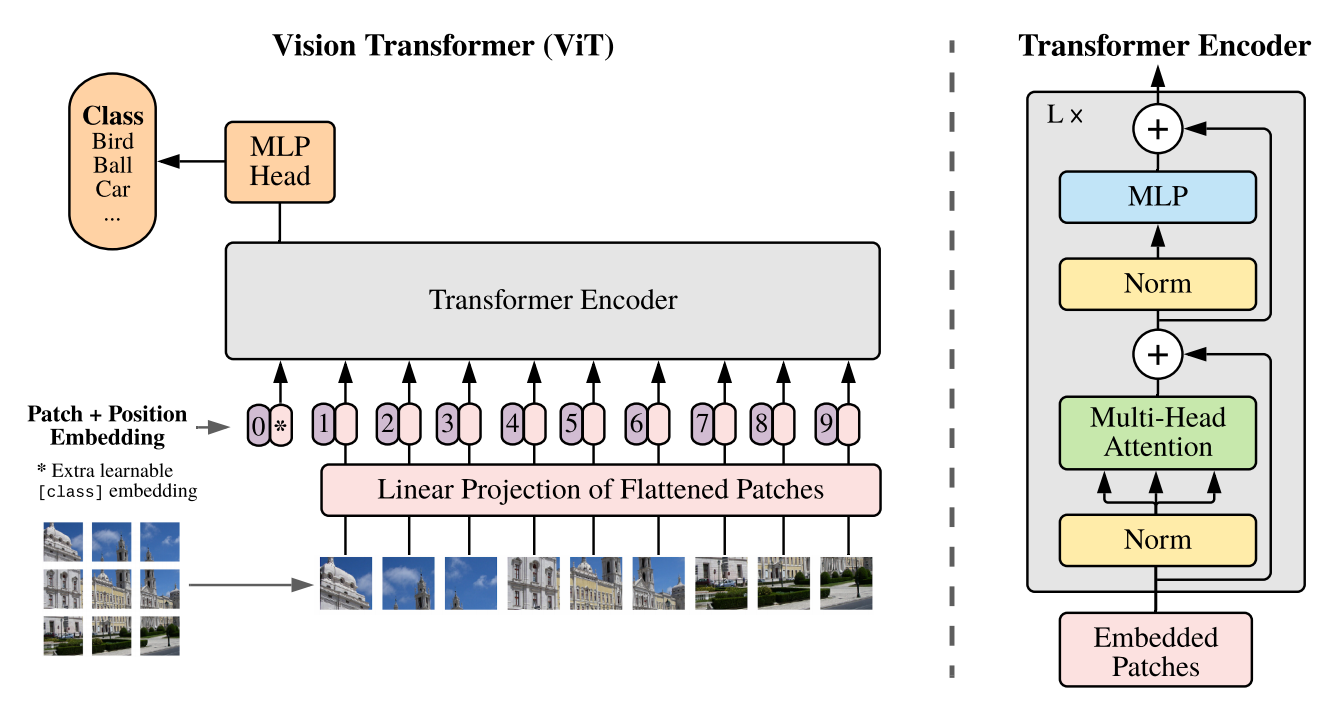
\includegraphics[scale=0.55]{ViT.png}
    \caption{ViT 架构}
    % \label{fig:fine}
\end{figure}
ViT 是一种将 Transformer 应用于图像分类任务的新型架构。Transformer 最初在自然语言处理(NLP)任务中取得了巨大成功,ViT则将其应用于计算机视觉领域,通过将图像划分为一系列图像块(patch),并将这些图像块视为序列数据进行处理。ViT 在许多图像分类任务上表现出色,特别是在大型数据集上。

ViT 的核心思想是将图像分割成固定大小的图像块,然后将这些图像块展平并嵌入到更高维度的向量空间中。每个图像块通过线性变换被映射为一个特征向量,这些特征向量连同位置编码一起作为 Transformer 编码器的输入。

具体步骤如下:
\begin{enumerate}
    \item 图像分割:将输入图像 $x \in \mathbb{R}^{H \times W \times C}$ 划分为 $N$ 个不重叠的图像块,每个图像块的大小为 $P \times P$,因此 $N = \frac{HW}{P^2}$。
    \item 图像块展平和嵌入:将每个图像块展平并通过线性变换映射到$d$维特征向量,得到 $z_0 \in \mathbb{R}^{N \times d}$。
    \item 位置编码:为每个图像块添加位置编码,以保留空间位置信息,位置编码与特征向量相加形成最终输入 $z_0 + E_{pos}$。
    \item Transformer 编码器:将上述输入序列传递给标准的 Transformer 编码器,编码器由多层自注意力机制和前馈神经网络组成。
    \item 分类:使用分类标记(class token)作为输入序列的一部分,通过 Transformer 编码器的输出进行图像分类。
\end{enumerate}
ViT 在大型数据集上的表现优异,并且在参数数量相近的情况下,能够比传统卷积神经网络取得更好的性能。其主要优势包括:
\begin{itemize}
    \item 灵活性:ViT 能够处理不同分辨率和大小的图像,只需调整图像块的大小即可。
    \item 全局信息:自注意力机制能够捕捉图像中的全局信息,而不是局限于局部感受野。
    \item 可扩展性:ViT 能够轻松扩展到更大的模型尺寸和更多的参数,从而进一步提高性能。
\end{itemize}
然而,ViT的一个主要挑战是在小型数据集上容易过拟合,因此在使用 ViT 时,通常需要预训练模型或更强的数据增强技术(如 Cutmix)。

\subsection{模型参数量估计}


\subsection{优化器设置}
两种架构的优化器都选择 Adam 优化器。除学习率和权重衰退以外,其余参数都为默认参数。


\section{调参结果}
本实验调节两个参数以尽可能提高模型性能:学习率 \texttt{lr} 和权重衰退 \texttt{weight\_decay}.

经过多轮调参,最终确定 resnet18 的 \texttt{lr} 为1e-3,\texttt{weight\_decay} 为0. ViT 的 \texttt{lr} 为4e-4,\texttt{weight\_decay} 为1e-5.


\section{实验结果}
\subsection{数据分析}
以下图片中,\textcolor{orange}{橙线}都是 \textcolor{orange}{resnet18 网络}的数据曲线,\textcolor{blue}{蓝线}都是 \textcolor{blue}{ViT 网络}的数据曲线.

\begin{figure}[H]
    \centering
    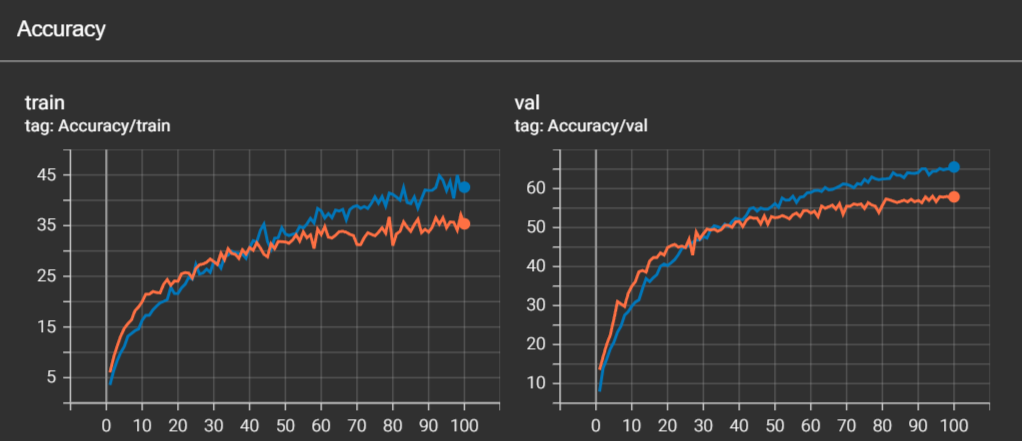
\includegraphics[scale=0.75]{transformer_acc.png}
    \caption{准确率对比}
    % \label{fig:acc}
\end{figure}
可以看出两个模型的准确率在训练的过程中不断上升,并且都没有饱和,理论上如果训练更长时间,两者都能获得更好的效果。训练初始阶段 resnet18 性能更好,约30个 epoch 左右被 ViT 超越。resnet18 的最终验证集准确率为57.88\%,ViT的最终验证集准确率为65.53\%.
\begin{figure}[H]
    \centering
    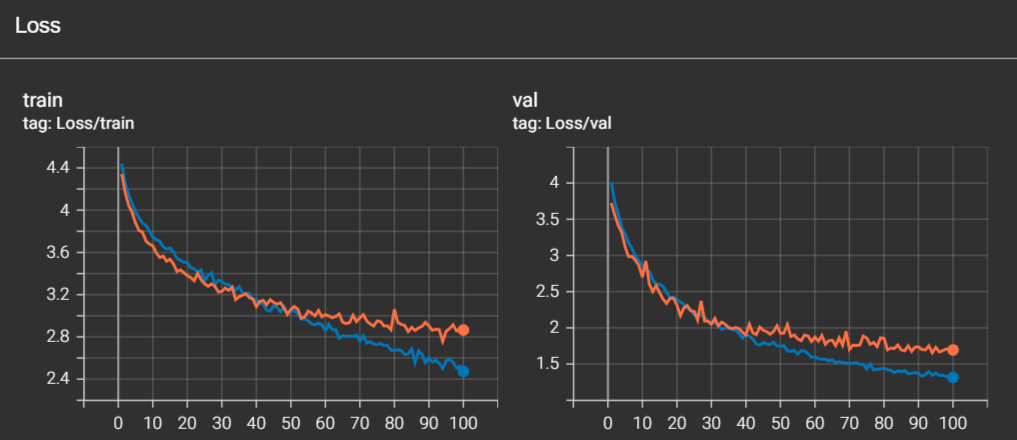
\includegraphics[scale=0.75]{transformer_loss.png}
    \caption{损失函数对比}
    % \label{fig:loss}
\end{figure}
两个模型的损失函数值也逐渐下降,初始时 resnet18 下降更快,但随后被 ViT 超越。



\subsection{结论}
以上实验结果一定程度上验证了 ViT 原论文中的结论,即 ViT 虽然在较小的数据集上性能不如 CNN 网络,但在更大的数据集上,ViT 的性能可以超越 CNN 架构。在我们的实验中,可以认为训练轮数较少等价于数据集较小,因此随着训练的进行,模型学习的数据量增多,ViT 的性能逐渐超越 resnet18.

以下是 ViT 原论文中两种模型的性能对比,其中 BiT 是一种基于CNN的模型架构,灰色区域是其架构的性能范围,随着数据量的增加,ViT 的性能增加比BiT更多。

\begin{figure}[H]
    \centering
    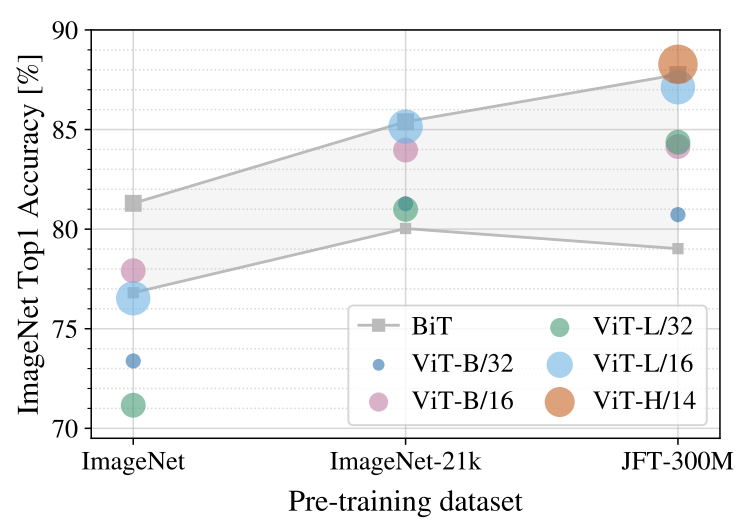
\includegraphics[scale=0.75]{ViT_vs_CNN.png}
    \caption{数据集大小与模型性能的关系}
    % \label{fig:loss}
\end{figure}

ViT 由于其较复杂的结构,在小数据集和短期训练中容易过拟合,导致其性能不如 resnet18。但随着训练数据量的增加,ViT 能够更好地利用其全局注意力机制,捕捉数据中的长距离依赖关系,从而逐渐提升其性能。在相同训练策略下,ViT 需要更多的训练时间和数据量来展现其优势。因此,在实际应用中,为了充分发挥 ViT 的潜力,通常需要结合大规模数据集或进行预训练。对于数据量有限的任务,resnet18 等传统 CNN 架构依然是有效的选择。而对于数据量充足的任务,ViT 则展现出更强的性能和泛化能力。

\chapter{基于 NeRF 的物体重建和新视图合成3}
\section{任务描述}
\begin{enumerate}
\item 选取身边的物体拍摄多角度图片/视频,并使用COLMAP估计相机参数,随后使用现成的框架进行训练;
\item 基于训练好的NeRF渲染环绕物体的视频,并在预留的测试图片上评价定量结果。
\end{enumerate}

\section{实验设置}

\section{项目架构}

\section{实验结果}


\end{document}
